
\begin{center}
{\includegraphics[scale=1.5]{om.eps}}
\end{center}

೧ ``ಸತ್ಯಜ್ಞಾನಾನಂತಬ್ರಹ್ಮನೂ, ಭಾರತೀಭರತಾಚಾರ್ಯನೂ, ವಿದ್ಯಾರಾಜನು, ಜ್ಞಾನಯಜ್ಞಾಮುದ್ರನ್ವಿತನೂ, ಹಂಸವಿಜ್ಞಾನೋಪದೇಶಕನೂ, ಅಮೃತರಸಧಾರೆಯನ್ನು ಹರಿಸುತ್ತಾ ವಿಶ್ವಭರತಕ್ಕೆ  ಶ್ರೇಯಃ-ಪ್ರೇಯಸ್ಸುಗಳನ್ನು ನೀಡುತ್ತಿರುವ ಪ್ರಣವಹಯಹಂಸಪರೋರಜನೂ ಆದ ಶ್ರೀಮನ್ನಾರಾಯಣನ ಶುಡರಡಿಗಳಲ್ಲಿ ಪ್ರಾಣಗಳನ್ನು ಬಗ್ಗಿಸಿ ಪ್ರಣಾಮಮಾಡೋಣ.

೨ ``ತ್ರಿವಿಕ್ರಮವಿಷ್ಣುಲಕ್ಷ್ಮೀನಿಕೇತನವೂ, ಶಿವಶಕ್ತಿಸುಮಂದಿರವೂ ಆದ ಜ್ಞಾನ ವಿಜ್ಞಾನಮಂದಿರವ್ಯೋಮಾಂಬುಜದಲ್ಲಿ ಮಹರ್ಷಿಗಳ ಅಂತರ್ಲಕ್ಪ್ಯಕ್ಕೆ ವೇದ್ಯನಾದ ಸರ್ವವಿದ್ಯಾಮೂಲಜ್ಯೋತಿಯನ್ನು ಕಂಡು ಭಾರತಭರತರೂ ಆನಂದಭರಿತರೂ ಆಗಿ ನಲಿಯುತ್ತಾ (ನಾಟ್ಯವಾದುತ್ತಾ) ನಮ್ಮ cಅತುಷ್ಪಷ್ಟಿಕಲೆಗಳಲ್ಲಿ ಹುದುಗಿರುವ ಆ ಜ್ಞಾನವಿಜ್ಞಾನಮಯಮಹಾಹಯಹಂಸಜ್ಯೋತಿಸ್ಸ್ತಂಭದ ಮೇಲಿರುವ ಮೂಲದೀಪದಿಮ್ದ ದೀಪಮಾಲಾಸಹಸ್ರವನ್ನು ವಿಶ್ವವಿಜ್ಞಾನಮಂದಿರದಲ್ಲಿ ಹಚ್ಚಿ (ಹತ್ತಿಸಿ) ಪ್ರಜ್ವಲಿಸುವಂತೆ ಮಾಡೋಣ.

೩. ``ಮಾಹಾಮಸ್ತಿಷ್ಕವೆಂಬ ಜ್ಞಾನವಿಜ್ಞಾನಮಂದಿರದ ತ್ರಿಧಾಮಯುತವಾದ ಬ್ರಹ್ಮಮಾರ್ಗತತ್ತ್ವಸೋಪಾನವಿಶ್ವರಂಗಾಂಬುಜದಲ್ಲಿ ಹಂಸಾಸನೆಯಾಗಿ, ಹಂಸ ಗಮನೆಯಾಗಿ ನಾದಶಬ್ದಬ್ರಹ್ಮರೂಪಿಣಿಯಾಗಿ, ಬ್ರಹ್ಮದಂಡನೀತಿಯನ್ನು ವಿವರಿಸುವ ತ್ರಿಕಾಲನಾಡಿಮೂರ್ತಿಸುಮ್ದರಿಯಾಗಿ, ಪ್ರಮಬ್ರಹ್ಮಗೃಹಿಣಿಯಾಗಿ, ವೇದಗರ್ಭೆಯಾಗಿ, ವಿಶ್ವಚೈತನ್ಯಸ್ತನ್ಯದಾಯಿನಿಯಾಗಿ, ಜೀವಸುಮನಸವನ್ನರಳಿಸುವ ಪ್ರಾಣಶಕ್ತಿಯಾಗಿ, ಬ್ರಹ್ಮಭಾವಜ್ಯೋತಿರ್ನಾದವಿಜ್ಞಾನವಿಪಂಚಿಕೆಯನ್ನು ಪ್ರಪಂಚಿಸಿ ಆತ್ಮಶ್ರೀಯನ್ನು ಬೀರುವವಳಾಗಿ, ನಮ್ಮ ಮಂದಿರದ, ಹೃತ್ಮಂದಿರದ ಮಹಾಮಂಗಳಾದೀಪರೇಖೆಯೂ, ವಿದ್ಯಾರಾಣಿಯೂ, ವಿಶ್ವಶಿಲ್ಪವಿಧಾನಜ್ಞೆಯೂ ಆದ ಮಹಾನಾಟ್ಯಭಾರತಿಯ ಪದಪುಂಡರೀಕಮಹಾಮಧುವನ್ನು ನಮ್ಮ ಪ್ರಾಣ ಮಧುಕರವು ಪೂರ್ಣಚಂದ್ರಿಕೆಯಲ್ಲಿ ನಿರನ್ತರವಾಗಿ (ಸದಾ) ಪಾನ ಮಾಡುತ್ತಿರಲಿ."

\vskip 20pt
\centerline{{\bf ಓಂ ತತ್ ಸತ್}}
